\documentclass[aspectratio=169]{beamer}
\usetheme{Madrid}
\usecolortheme{default}
\setbeamertemplate{navigation symbols}{}
\usepackage[utf8]{inputenc}
\usepackage{amsmath,amssymb}
\usepackage{tikz}
\usetikzlibrary{arrows.meta,positioning}
\usepackage{hyperref}

\title[Bitcoin Transaction Classification]{Bitcoin Transaction Classification}
\author{Sanchayan Bhowal}
\date{sbhowal@stanford.edu}

\definecolor{mygreen}{RGB}{46,125,50}
\definecolor{myred}{RGB}{198,40,40}
\definecolor{myblue}{RGB}{30,70,140}

\begin{document}

\begin{frame}
    \titlepage
\end{frame}

\begin{frame}{Problem and Data}
    \begin{columns}[T,onlytextwidth]
        \column{0.57\textwidth}
        \textbf{Goal:} classify Bitcoin transaction entities as \alert{illicit} or \textcolor{mygreen}{licit}.

        \vspace{0.5em}
        \textbf{Why this is hard}
        \begin{itemize}
            \item Observed labels may be noisy.
            \item Transactions linked in the network are not independent (illicit transactions may cluster together through payment flows.)
        \end{itemize}

        \vspace{0.4em}
        \textbf{Dataset:} Elliptic Bitcoin dataset
        \begin{itemize}
            \item $>$200K transaction entities (nodes)
            \item 234K payment flows (edges)
            \item 166 node features ($X_i$)
        \end{itemize}

        \column{0.43\textwidth}
        \centering
        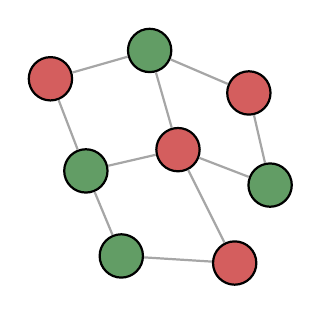
\begin{tikzpicture}[scale=0.9, every node/.style={circle, draw=black, thick, minimum size=0.55cm, inner sep=0pt}]
            \node[fill=myred!75] (a) at (0.2,2.5) {};
            \node[fill=mygreen!75] (b) at (1.6,2.9) {};
            \node[fill=myred!75] (c) at (3.0,2.3) {};
            \node[fill=mygreen!75] (d) at (0.7,1.2) {};
            \node[fill=myred!75] (e) at (2.0,1.5) {};
            \node[fill=mygreen!75] (f) at (3.3,1.0) {};
            \node[fill=mygreen!75] (g) at (1.2,0.0) {};
            \node[fill=myred!75] (h) at (2.8,-0.1) {};

            \draw[thick, gray!70] (a) -- (b);
            \draw[thick, gray!70] (b) -- (c);
            \draw[thick, gray!70] (a) -- (d);
            \draw[thick, gray!70] (d) -- (e);
            \draw[thick, gray!70] (b) -- (e);
            \draw[thick, gray!70] (c) -- (f);
            \draw[thick, gray!70] (d) -- (g);
            \draw[thick, gray!70] (e) -- (h);
            \draw[thick, gray!70] (g) -- (h);
            \draw[thick, gray!70] (e) -- (f);
        \end{tikzpicture}

        \vspace{0.5em}

        \footnotesize
        \textcolor{myred!75}{\rule{0.5em}{0.5em}} illicit \qquad
        \textcolor{mygreen!75}{\rule{0.5em}{0.5em}} licit
    \end{columns}
\end{frame}

\begin{frame}{Probabilistic Model}
    \textbf{Step 1: noisy observed labels}
    \[
        P(y_i\mid \sigma_i)=
        \begin{cases}
            1-\epsilon, & y_i=\sigma_i,     \\
            \epsilon,   & y_i\neq \sigma_i,
        \end{cases}
    \]
    where $\sigma_i$ is the true label and $y_i$ is the observed label.

    \vspace{0.7em}
    \textbf{Step 2: dependence through the network}
    \[
        P(\sigma_1,\sigma_2,\ldots,\sigma_n\mid X,G)
        \propto
        \prod_{(i,j)\in E} \psi_{X_i,X_j}(\sigma_i,\sigma_j).
    \]

    \begin{itemize}
        \item $\psi_{X_i,X_j}$ is a \textbf{symmetric compatibility score} for two connected transactions.
    \end{itemize}

    \begin{block}{Aim}
        Infer the distribution of true labels $\sigma_i$ given observed labels $y_i$, features $X_i$, and graph structure $G$.
    \end{block}

\end{frame}

\begin{frame}{Why This Framing?}
    \begin{block}{Main idea}
        Use a probabilistic graphical model to combine \textbf{feature information}, \textbf{network dependence}, and \textbf{label uncertainty} in one framework.
    \end{block}

    \vspace{0.5em}
    \textbf{Compared with standard approaches}
    \begin{itemize}
        \item Logistic regression is interpretable, but ignores graph dependence.
        \item Machine learning methods use the graph, but lack interpretability.
    \end{itemize}
\end{frame}

\end{document}
